\documentclass[a4paper,11pt]{article}

\usepackage{amsmath}
\usepackage{amssymb}
\usepackage[english]{babel}
\usepackage[style=ieee,backend=bibtex]{biblatex}
\usepackage{booktabs}
\usepackage[font={small},labelfont=sc]{caption}
\usepackage[hidelinks]{hyperref}
\usepackage{fancyhdr}
\usepackage{float}
\usepackage[symbol]{footmisc}
\usepackage[margin=1in]{geometry}
\usepackage{graphicx}
\usepackage[latin1]{inputenc}
\usepackage{listings}
\usepackage{mathtools}
\usepackage{microtype}
\usepackage{multirow}
\usepackage{rotating}
\usepackage{siunitx}
\usepackage{subcaption}
\usepackage{threeparttable}
\usepackage{tikz,pgfplots}
    \pgfplotsset{compat=1.15,set layers}
    \usetikzlibrary{calc}
    \usetikzlibrary{external}
    	\tikzexternalize[prefix=tikz/]
	\usetikzlibrary{fit}
	\usetikzlibrary{positioning}
    \usetikzlibrary{quotes}
	\usetikzlibrary{shapes.misc}
	\pgfdeclarelayer{background}
	\pgfdeclarelayer{foreground}
	\pgfsetlayers{background,main,foreground}
\usepackage{titling}
\usepackage{xspace}

\newcommand{\Altera}{\textsc{Altera}\textsuperscript{\textregistered}\xspace}
\newcommand{\QuartusII}{Quartus\textsuperscript{\textregistered} \textsc{ii}\xspace}

\title{Carry Select Adder Design in VHDL and \Altera \QuartusII}
\author{Z0996690}
\date{\today}

\pagestyle{fancy}
\fancyhf{}
\lhead{
\includegraphics[width=0.1\textwidth]{img/Durham.png}}
\chead{\thetitle}
\rhead{\theauthor}
\cfoot{\thepage}

% Listings preamble
\definecolor{codegreen}{rgb}{0,0.6,0}
\definecolor{codegray}{rgb}{0.5,0.5,0.5}
\definecolor{codepurple}{rgb}{0.58,0,0.82}
\definecolor{backcolour}{rgb}{0.95,0.95,0.92}

\lstdefinestyle{mystyle}{
    % backgroundcolor=\color{backcolour},
    commentstyle=\color{codegreen},
    keywordstyle=\color{magenta},
    numberstyle=\tiny\color{codegray},
    stringstyle=\color{codepurple},
    rulecolor=\color{codegray},
    % rulesepcolor=\color{codegray},
    basicstyle=\ttfamily\scriptsize,
    breakatwhitespace=false,
    breaklines=true,
    captionpos=b,
    keepspaces=true,
    numbers=left,
    numbersep=5pt,
    showspaces=false,
    showstringspaces=false,
    showtabs=false,
    tabsize=4,
	frame=single,
	frameround=tttt
}

\begin{document}

% Abstract
\begin{@twocolumnfalse} \centering
    \renewcommand{\abstractname}{\large Abstract}
    \begin{abstract}
        This report describes the design and evalation of a 32-bit Carry Select Adder (CSA), evaluating how it compares to the conventional Carry Ripple Adder (CRA) in timing, complexity and implementation area.
    \end{abstract}
\end{@twocolumnfalse}

\section{Circuits and Coding}

Carry Ripple Adders (CRA) are an example of iterative logic where the carry out of each full adder comprises the intercell signal. Iterative logic circuits are easy to implement and test, and subsequently the first adders were built this way. A downside of iterative logic is the time for the intercell signal to propagate to the last iterative unit.

Carry Select Adders (CSA) are fast adders which aim to reduce propagation delay by performing much of the computation in parallel. A schematic of a 32-bit CSA is detailed in Figure~\ref{fig:csa}.

\begin{figure}[!h]
	\centering
	\hspace{-\textwidth}
	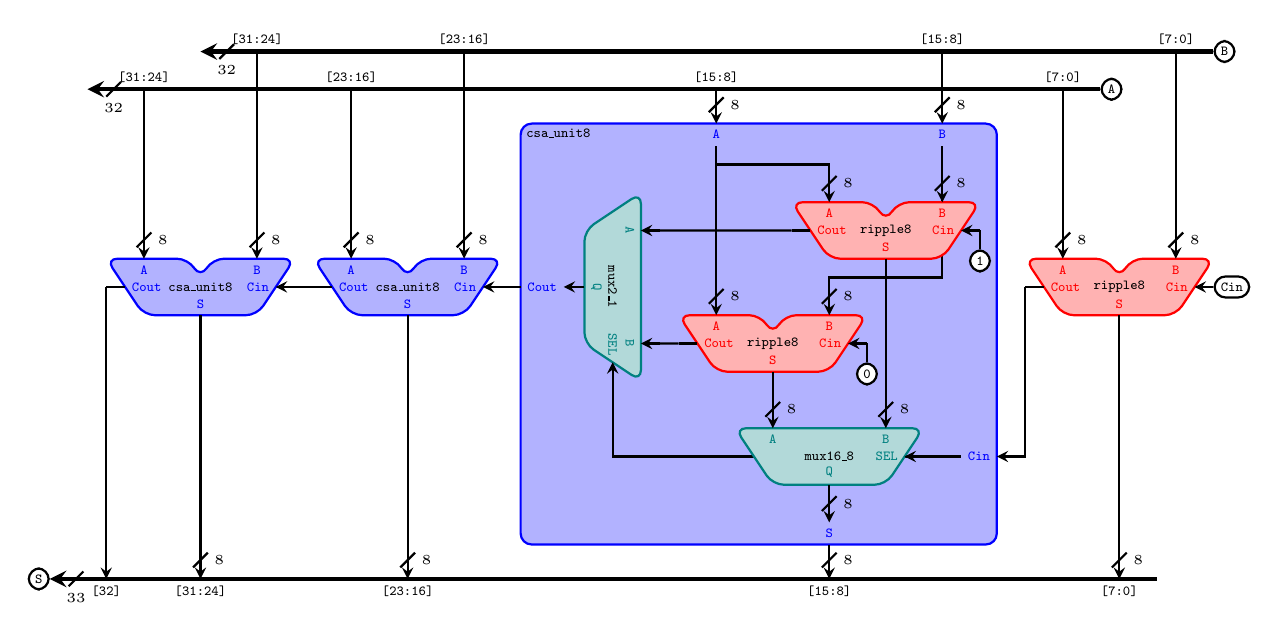
\begin{tikzpicture}[
		>=stealth,
		multiplexer/.pic={
			\coordinate (-O) at (0,0);
			\coordinate (-A) at (-3em,2.5em);
			\coordinate (-B) at (3em,2.5em);
			\coordinate (-SEL) at (5em,0);
			\coordinate (-Q) at (0,-2.5em);
			\draw [pic actions] (-3em,-1.5em) -- (3em,-1.5em) -- (5em,1.5em) -- (-5em,1.5em) --cycle;
			\draw [->,pic actions,fill=black,draw=black] (-A) -- (-3em,1.5em);
			\draw [->,pic actions,fill=black,draw=black] (-B) -- (3em,1.5em);
			\draw [->,pic actions,fill=black,draw=black] (-SEL) -- (4em,0);
			\draw [pic actions,draw=black] (0,-1.5em) -- (-Q);
			\node [anchor=center,text=black] (-center) {\tt\tikzpictext};
			\begin{pgfonlayer}{foreground}
				\node [anchor=north] at (-3em,1.5em) {\tiny\tt{A}};
				\node [anchor=north] at (3em,1.5em) {\tiny\tt{B}};
				\node [anchor=south] at (0,-1.5em) {\tiny\tt{Q}};
				\node [anchor=east] at (4em,0) {\tiny\tt{SEL}};
			\end{pgfonlayer}
	  	},
		adder/.pic={
			\coordinate (-O) at (0,0);
			\coordinate (-A) at (-3em,2.5em);
			\coordinate (-B) at (3em,2.5em);
			\coordinate (-Cin) at (5em,0);
			\coordinate (-Cout) at (-5em,0);
			\coordinate (-S) at (0,-2.5em);
			\draw [pic actions] (-3em,-1.5em) -- (3em,-1.5em) -- (5em,1.5em) -- (0.66em,1.5em) -- (0,0.5em) -- (-0.66em,1.5em) -- (-5em,1.5em) --cycle;
			\draw [->,pic actions,fill=black,draw=black] (-A) -- (-3em,1.5em);
			\draw [->,pic actions,fill=black,draw=black] (-B) -- (3em,1.5em);
			\draw [->,pic actions,fill=black,draw=black] (-Cin) -- (4em,0);
			\draw [pic actions,fill=black,draw=black] (-4em,0) -- (-Cout);
			\draw [pic actions,draw=black] (0,-1.5em) -- (-S);
			\node [anchor=center,text=black] (-center) {\tt\tikzpictext};
			\begin{pgfonlayer}{foreground}
				\node [anchor=north] at (-3em,1.5em) {\tiny\tt{A}};
				\node [anchor=north] at (3em,1.5em) {\tiny\tt{B}};
				\node [anchor=south] at (0,-1.5em) {\tiny\tt{S}};
				\node [anchor=east] at (4em,0) {\tiny\tt{Cin}};
				\node [anchor=west] at (-4em,0) {\tiny\tt{Cout}};
			\end{pgfonlayer}
	  	}
	]\tiny
		\pic ["mux16\_8",thick,draw=teal,fill=teal!30,text=teal,rounded corners] (smux) {multiplexer};

		\node [draw,strike out,thick,minimum size=0.1] (bus-S0) at (smux-A) {};
		\node [draw,strike out,thick,minimum size=0.1] (bus-S1) at (smux-B) {};
		\node [draw,strike out,thick,minimum size=0.1] (bus-S) at (smux-Q) {};
		\node [anchor=west] at (bus-S0.east) {8};
		\node [anchor=west] at (bus-S1.east) {8};
		\node [anchor=west] at (bus-S.east) {8};

		\pic ["ripple8",thick,draw=red,fill=red!30,text=red,rounded corners,above=3.5em of smux-A] (ra0) {adder};

		\node [draw,strike out,thick,minimum size=0.1] (bus-A) at (ra0-A) {};
		\node [draw,strike out,thick,minimum size=0.1] (bus-B) at (ra0-B) {};
		\node [anchor=west] at (bus-A.east) {8};
		\node [anchor=west] at (bus-B.east) {8};

		\pic ["ripple8",thick,draw=red,fill=red!30,text=red,rounded corners,above=9.5em of smux-B] (ra1) {adder};

		\node [draw,strike out,thick,minimum size=0.1] (bus-A) at (ra1-A) {};
		\node [draw,strike out,thick,minimum size=0.1] (bus-B) at (ra1-B) {};
		\node [anchor=west] at (bus-A.east) {8};
		\node [anchor=west] at (bus-B.east) {8};

		\pic ["mux2\_1",thick,draw=teal,fill=teal!30,text=teal,rounded corners,rotate=-90,transform shape,left=6.5em of $(ra0-Cout)!0.5!(ra1-Cout)$] (cmux) {multiplexer};

		\node [draw,fill=white,thick,rectangle,rounded corners,below=1em of ra0-Cin] (0) {\tt{0}};
		\node [draw,fill=white,thick,rectangle,rounded corners,below=1em of ra1-Cin] (1) {\tt{1}};

		\node [text=blue,above=8em of ra0-A] (unit1-A) {\tt{A}};
		\node [text=blue,above=2em of ra1-B] (unit1-B) {\tt{B}};
		\node [text=blue,right=2em of smux-SEL] (unit1-Cin) {\tt{Cin}};

		\node [text=blue,left=0.1em of cmux-Q] (unit1-Cout) {\tt{Cout}};
		\node [text=blue,below=1em of smux-Q] (unit1-S) {\tt{S}};

		\begin{pgfonlayer}{background}
			\node [draw=blue,fill=blue!30,thick,rectangle,rounded corners,inner sep=0,fit=(unit1-A) (unit1-B) (unit1-Cin) (unit1-Cout) (unit1-S)] (unit1) {};

			\node [anchor=north west,rounded corners,rectangle] at (unit1.north west) {\tt{csa\_unit8}};

			\draw [thick] (ra0-Cin) -- (0);
			\draw [thick] (ra1-Cin) -- (1);

			\draw [thick] (ra0-A) -- (unit1-A);
			\draw [thick] (ra1-A) -- ($(ra1-A) + (0,1em)$) -| (unit1-A);

			\draw [thick] (ra0-B) -- ($(ra0-B) + (0,1em)$) -| (unit1-B);
			\draw [thick] (ra1-B) -- (unit1-B);

			\draw [thick] (ra0-S) -- (smux-A);
			\draw [thick] (ra1-S) -- (smux-B);

			\draw [thick] (ra0-Cout) -- (cmux-B);
			\draw [thick] (ra1-Cout) -- (cmux-A);

			\draw [thick] (cmux-SEL) |- (unit1-Cin);
			\draw [thick] (smux-SEL) -- (unit1-Cin);

			\draw [->,thick] (cmux-Q) -- (unit1-Cout);
			\draw [->,thick] (smux-Q) -- (unit1-S);
		\end{pgfonlayer}

		\pic ["ripple8",thick,draw=red,fill=red!30,text=red,rounded corners,right=29.5em of unit1-Cout] (unit0) {adder};

		\pic ["csa\_unit8",thick,draw=blue,fill=blue!30,text=blue,rounded corners,left=6em of unit1-Cout] (unit2) {adder};
		\pic ["csa\_unit8",thick,draw=blue,fill=blue!30,text=blue,rounded corners,left=6em of unit2-Cout] (unit3) {adder};

		\node [above=8em of unit3-A] (A3) {\tiny\tt{[31:24]}};
		\node [above=8em of unit2-A] (A2) {\tiny\tt{[23:16]}};
		\node [above=3em of unit1-A.south] (A1) {\tiny\tt{[15:8]}};
		\node [above=8em of unit0-A] (A0) {\tiny\tt{[7:0]}};
		\node [left=3em of A3.south] (A-end) {};
		\node [draw,thick,rectangle,rounded corners,right=2em of A0.south] (A-start) {\tt{A}};

		\node [above=10em of unit3-B] (B3) {\tiny\tt{[31:24]}};
		\node [above=10em of unit2-B] (B2) {\tiny\tt{[23:16]}};
		\node [above=5em of unit1-B.south] (B1) {\tiny\tt{[15:8]}};
		\node [above=10em of unit0-B] (B0) {\tiny\tt{[7:0]}};
		\node [left=3em of B3.south] (B-end) {};
		\node [draw,thick,rectangle,rounded corners,right=2em of B0.south] (B-start) {\tt{B}};

		\node [below=15.5em of unit3-Cout] (S4) {\tiny\tt{[32]}};
		\node [below=13em of unit3-S] (S3) {\tiny\tt{[31:24]}};
		\node [below=13em of unit2-S] (S2) {\tiny\tt{[23:16]}};
		\node [below=3em of unit1-S.north] (S1) {\tiny\tt{[15:8]}};
		\node [below=13em of unit0-S] (S0) {\tiny\tt{[7:0]}};
		\node [draw,thick,rectangle,rounded corners,left=3em of S4.north] (S-end) {\tt{S}};
		\node [right=2em of S0.north] (S-start) {};

		\node [draw,thick,rectangle,rounded corners,anchor=west] at (unit0-Cin) {\tt{Cin}};

		\node [draw,strike out,thick,minimum size=0.1] at (unit0-A) (bus-A) {};
		\node [draw,strike out,thick,minimum size=0.1] at (unit0-B) (bus-B) {};
		\node [draw,strike out,thick,minimum size=0.1,above=1em of S0,anchor=center] (bus-S) {};
		\node [anchor=west] at (bus-A.east) {8};
		\node [anchor=west] at (bus-B.east) {8};
		\node [anchor=west] at (bus-S.east) {8};

		\node [draw,strike out,thick,minimum size=0.1,above=1em of unit1-A,anchor=center] (bus-A) {};
		\node [draw,strike out,thick,minimum size=0.1,above=1em of unit1-B,anchor=center] (bus-B) {};
		\node [draw,strike out,thick,minimum size=0.1,above=1em of S1,anchor=center] (bus-S) {};
		\node [anchor=west] at (bus-A.east) {8};
		\node [anchor=west] at (bus-B.east) {8};
		\node [anchor=west] at (bus-S.east) {8};

		\node [draw,strike out,thick,minimum size=0.1] at (unit2-A) (bus-A) {};
		\node [draw,strike out,thick,minimum size=0.1] at (unit2-B) (bus-B) {};
		\node [draw,strike out,thick,minimum size=0.1,above=1em of S2,anchor=center] (bus-S) {};
		\node [anchor=west] at (bus-A.east) {8};
		\node [anchor=west] at (bus-B.east) {8};
		\node [anchor=west] at (bus-S.east) {8};

		\node [draw,strike out,thick,minimum size=0.1] at (unit3-A) (bus-A) {};
		\node [draw,strike out,thick,minimum size=0.1] at (unit3-B) (bus-B) {};
		\node [draw,strike out,thick,minimum size=0.1,above=1em of S3,anchor=center] (bus-S) {};
		\node [anchor=west] at (bus-A.east) {8};
		\node [anchor=west] at (bus-B.east) {8};
		\node [anchor=west] at (bus-S.east) {8};

		\node [draw,strike out,thick,minimum size=0.1,right=1em of A-end] (bus-A) {};
		\node [draw,strike out,thick,minimum size=0.1,right=1em of B-end] (bus-B) {};
		\node [draw,strike out,thick,minimum size=0.1,right=1em of S-end] (bus-S) {};
		\node [anchor=north] at (bus-A.south) {32};
		\node [anchor=north] at (bus-B.south) {32};
		\node [anchor=north] at (bus-S.south) {33};

		\begin{pgfonlayer}{background}
			\draw [->,ultra thick] (A-start) -- (A-end);
			\draw [->,ultra thick] (B-start) -- (B-end);
			\draw [->,ultra thick] (S-start) -- (S-end);

			\draw [->,thick] (unit0-Cout) |- (unit1-Cin);
			\draw [thick] (unit1-Cout) -- (unit2-Cin);
			\draw [thick] (unit2-Cout) -- (unit3-Cout);

			\draw [thick] (A0) -- (unit0-A);
			\draw [->,thick] (A1) -- (unit1-A);
			\draw [thick] (A2) -- (unit2-A);
			\draw [thick] (A3) -- (unit3-A);

			\draw [thick] (B0) -- (unit0-B);
			\draw [->,thick] (B1) -- (unit1-B);
			\draw [thick] (B2) -- (unit2-B);
			\draw [thick] (B3) -- (unit3-B);

			\draw [->,thick] (unit0-S) -- (S0);
			\draw [->,thick] (unit1-S) -- (S1);
			\draw [->,thick] (unit2-S) -- (S2);
			\draw [->,thick] (unit3-S) -- (S3);
			\draw [->,thick] (unit3-Cout) -- (S4);
		\end{pgfonlayer}
	\end{tikzpicture}
	\hspace{-\textwidth}
	\caption{Diagram of a 32-bit carry select adder.}
	\label{fig:csa}
\end{figure}

Figure~\ref{fig:hierarchy} illustrates the hierarchy of files used to build the 32-bit CSA in Figure~\ref{fig:csa} and a 32-bit carry ripple adder for comparison. Both The CSA and CRA were implemented in \Altera \QuartusII and shared as much VHDL as possible to avoid discrepencies in implementation efficiency. Only the top-level files used the \QuartusII block schematic file format.

\begin{figure}[!h]
	\centering
	\footnotesize
	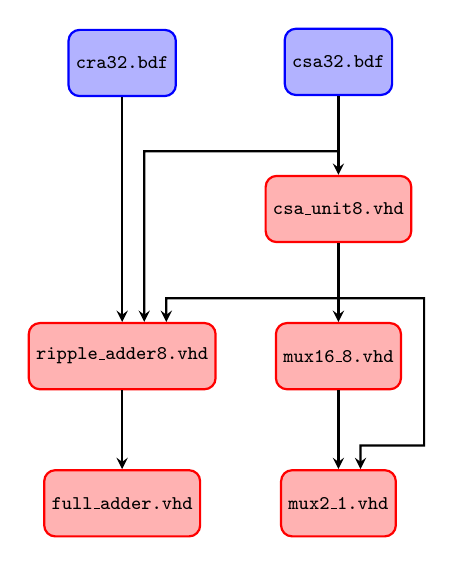
\begin{tikzpicture}[
		>=stealth,
		vhdl/.style={draw=red,fill=red!30,thick,rectangle,rounded corners,minimum size=3em},
		block/.style={draw=blue,fill=blue!30,thick,rectangle,rounded corners,minimum size=3em},
		inv/.style={draw=none,fill=none,rectangle,minimum size=3em}
	]\scriptsize
		\node [vhdl] (full_adder) {\texttt{full\_adder.vhd}};
		\node [vhdl,above=of full_adder] (ripple_adder8) {\texttt{ripple\_adder8.vhd}};
		\node [inv,above=of ripple_adder8] (inv) {};
		\node [block,above=of inv] (cra32) {\texttt{cra32.bdf}};

		\node [vhdl,right=of full_adder] (mux2_1) {\texttt{mux2\_1.vhd}};
		\node [vhdl,above=of mux2_1] (mux16_8) {\texttt{mux16\_8.vhd}};
		\node [vhdl,above=of mux16_8] (csa_unit8) {\texttt{csa\_unit8.vhd}};
		\node [block,above=of csa_unit8] (csa32) {\texttt{csa32.bdf}};

		\draw [->,thick] (mux16_8) -- (mux2_1);
		\draw [->,thick] (csa_unit8) -- (mux16_8);
		\draw [->,thick] (csa_unit8)
			-- ($(csa_unit8.south)!0.7!(mux16_8.north)$)
			-| ($(ripple_adder8.north) + (2em,0)$);
		\draw [->,thick] (csa_unit8)
			-- ($(csa_unit8.south)!0.7!(mux16_8.north)$)
			-| ($(mux16_8.east) + (1em,0)$)
			|- ($(mux16_8.south)!0.7!(mux2_1.north) + (1em,0)$)
			-- ($(mux2_1.north) + (1em,0)$);
		\draw [->,thick] (csa32) -- (csa_unit8);
		\draw [->,thick] (csa32)
			-- ($(csa32.south)!0.7!(csa_unit8.north)$)
			-| ($(ripple_adder8.north) + (1em,0)$);

		\draw [->,thick] (cra32) -- (ripple_adder8);
		\draw [->,thick] (ripple_adder8) -- (full_adder);
	\end{tikzpicture}
	\caption{Hierarchy of entity declarations.}
	\label{fig:hierarchy}
\end{figure}

Listings~\ref{lst:full_adder}~and~\ref{lst:mux2_1} include the logic expression used to implement the \texttt{full\_adder} and \texttt{mux2\_1} design entities.

\begin{center}
	\hspace{-\textwidth}%
	\begin{minipage}{0.6\textwidth}
		\lstinputlisting[
			caption={Architecture declaration in \texttt{full\_adder.vhd}},
			label={lst:full_adder},
			language=VHDL,
			style=mystyle,
			firstline=17,
			firstnumber=17,
		]{../quartus/full_adder.vhd}
	\end{minipage}%
	\hspace{2em}%
	\begin{minipage}{0.51\textwidth}
		\lstinputlisting[
			caption={Architecture declaration in \texttt{mux2\_1.vhd}},
			label={lst:mux2_1},
			language=VHDL,
			style=mystyle,
			firstline=16,
			firstnumber=16,
		]{../quartus/mux2_1.vhd}
	\end{minipage}%
	\hspace{-\textwidth}

\end{center}

The 16-to-8 multiplexor was constructed using eight parallel \texttt{mux2\_1} components, mapped to the elements of \texttt{std\_logic\_vector(7 downto 1)} type ports. A similar approach in Listing~\ref{lst:ripple_adder8} shows how intercell signals were used to connect \texttt{full\_adder} components together to build the 8-bit ripple adder design entity.

Signals were also used to represent the candidate sum and carry out values from the two 8-bit ripple adders detailed in the unit cells in Figure~\ref{fig:csa}. The VHDL implementation of the CSA unit cell is described in Listing~\ref{lst:csa_unit8}.

\begin{center}
	\hspace{-\textwidth}%
	\begin{minipage}{0.51\textwidth}
		\lstinputlisting[
			language=VHDL,
			style=mystyle,
			firstnumber=26,
			firstline=26,
			lastline=26
		]{../quartus/ripple_adder8.vhd}
		\lstinputlisting[
			label={lst:ripple_adder8},
			language=VHDL,
			style=mystyle,
			firstnumber=27,
			firstline=27,
			lastline=37
		]{../quartus/ripple_adder8.vhd}
		\lstinputlisting[
			caption={Snippet showing one of eight chained \texttt{full\_adder} components mapped in \texttt{ripple\_adder8.vhd} architecture declaration.},
			label={lst:ripple_adder8},
			language=VHDL,
			style=mystyle,
			firstnumber=63,
			firstline=63,
			lastline=68
		]{../quartus/ripple_adder8.vhd}
	\end{minipage}%
	\hspace{2em}%
	\begin{minipage}{0.57\textwidth}
		\lstinputlisting[
			language=VHDL,
			style=mystyle,
			firstnumber=44,
			firstline=44,
			lastline=47
		]{../quartus/csa_unit8.vhd}
		\lstinputlisting[
			caption={Snippet showing how the two ripple adders were mapped to the intermediate candidate signals before being selected using multiplexors and the carry in port in \texttt{csa\_unit8.vhd} architecture declaration.},
			label={lst:csa_unit8},
			language=VHDL,
			style=mystyle,
			firstnumber=48,
			firstline=48,
		]{../quartus/csa_unit8.vhd}
	\end{minipage}%
	\hspace{-\textwidth}

\end{center}

The top level design entities are shown in schematic in Figure~\ref{fig:top-level}

\begin{figure}[!h]
	\centering
	\footnotesize
	\begin{subfigure}[b]{\textwidth}
		\makebox[\textwidth][c]{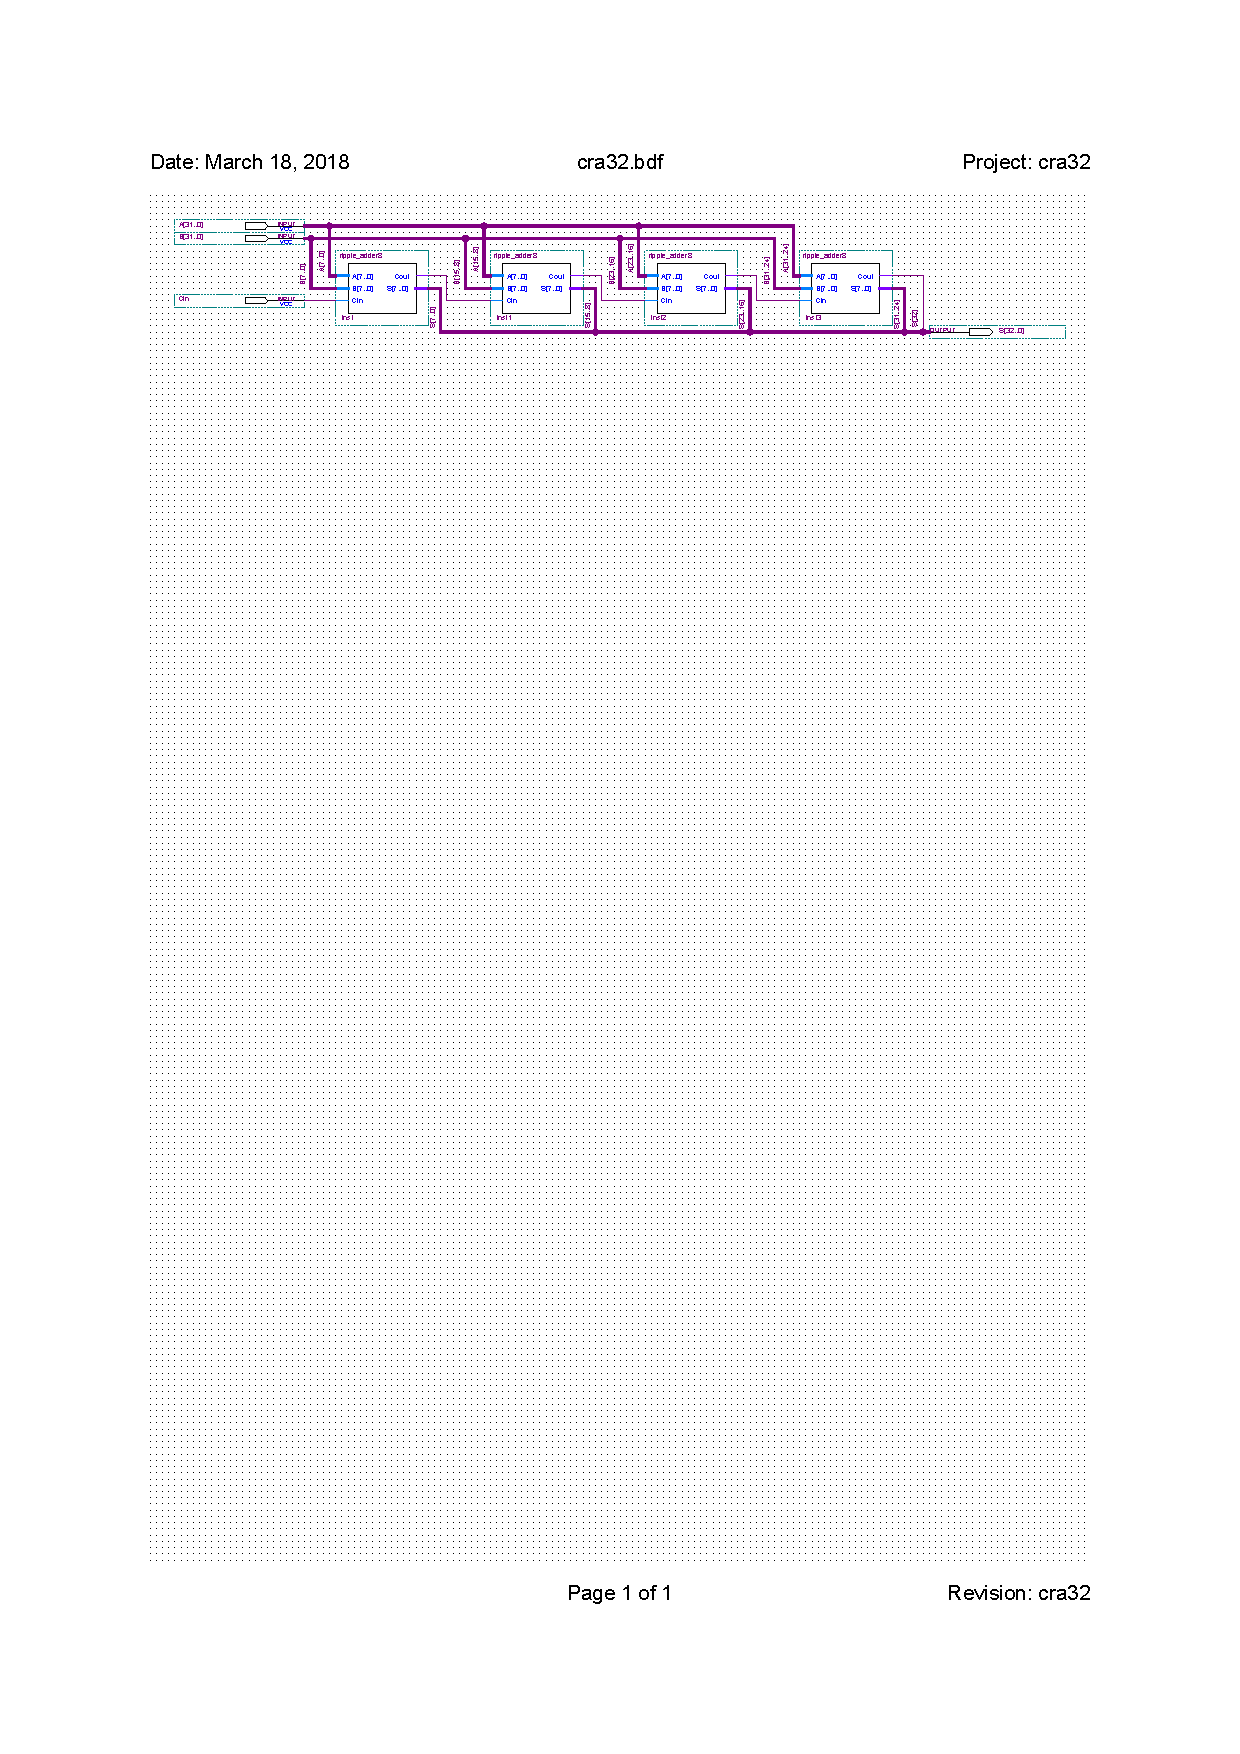
\includegraphics[width=1.3\textwidth,trim={82pt 680pt 82pt 104pt},clip]{results/cra32.pdf}}%
		\caption{\texttt{cra32.bdf}: 32-bit carry ripple adder}
		\label{fig:cra32.bdf}
	\end{subfigure}
	\begin{subfigure}[b]{\textwidth}
		\makebox[\textwidth][c]{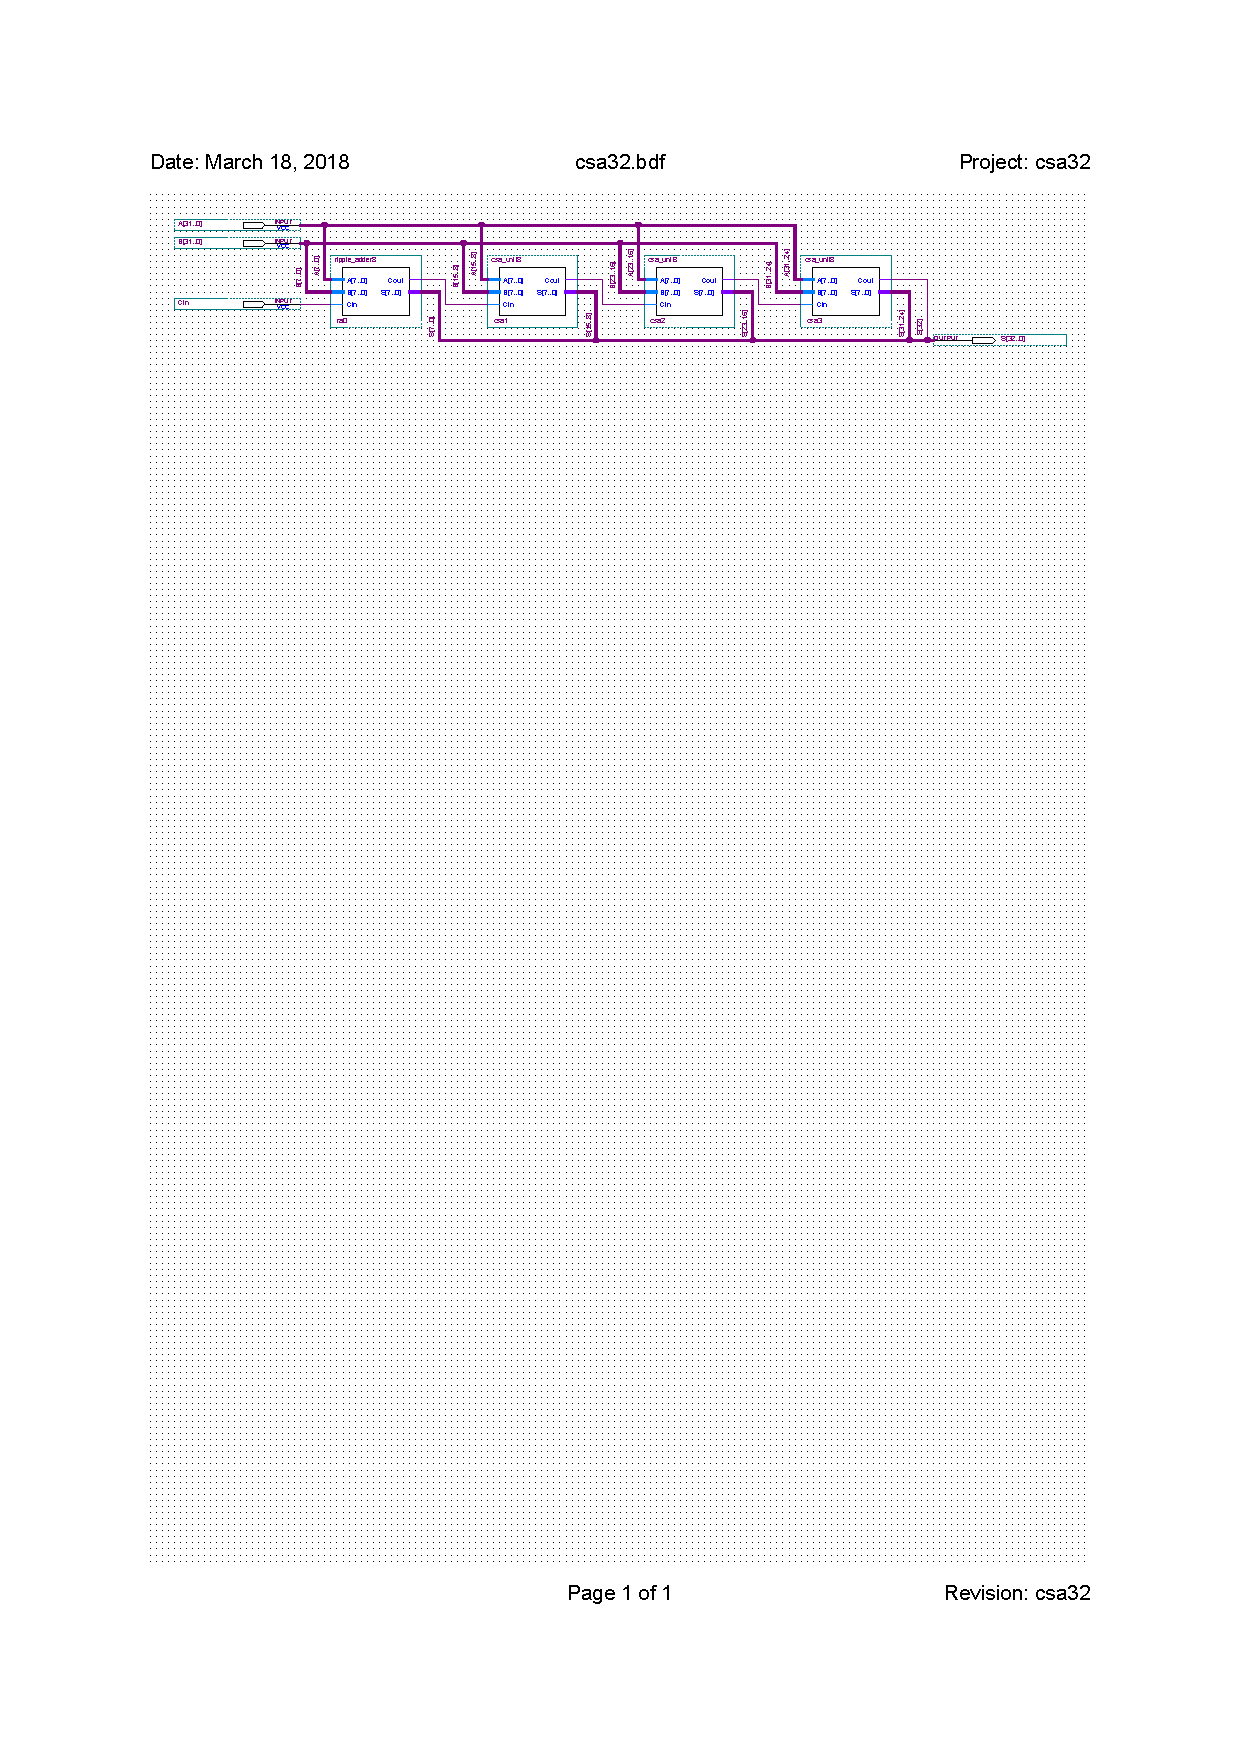
\includegraphics[width=1.3\textwidth,trim={82pt 678pt 82pt 104pt},clip]{results/csa32.pdf}}%
		\caption{\texttt{csa32.bdf}: 32-bit carry select adder, 8-bit select units}
		\label{fig:csa32.bdf}
	\end{subfigure}
	\caption{Block diagram schematics for the top-level entities of each project.}
	\label{fig:top-level}
\end{figure}

\section{Speed and Operation}

The 32-bit addition is split into 8-bit units which are executed in parallel. In each carry select unit, short ripple adders compute sum candidates for both possible carry in values. Simultaneously, the first intercell carry signal is computed by the inital adder. The intercell carry signals then propagate through the multiplexors selecting the correct sum and carry out candidates, rather than through the adders.

The propagation delay of the CSA is only as long as the 8-bit ripple adder and 3 multiplexors, much faster in theory than the propagation delay of a 32-bit ripple adder.

Apparent drawbacks of the CSA compared to the CRA include the increased complexity, size and power requirements due to duplicating most of the full adders and including multiplexors.

\section{FPGA Implementation}

\printbibliography

\end{document}